Because of its thin atmosphere, Mars has surface features which present analogies with both Moon, through the impact craters, and Earth, with volcanoes, deserts, polar ice caps. It is mainly composed of carbon dioxide $CO_2$ (96,0 \% $\pm$ 0,7 \%), argon $Ar$ (1,93 \% $\pm$ 0,01 \%) and oxygen
$O_2$ (0,145 \% $\pm$ 0,009 \%). As the gravity of Mars is low, the height of the atmosphere is 11 km, more than one and a half times higher than the Earth's one (7 km). Moreover, due to this low gravity, the wind can disrupt a rover easier than on Earth and a large amount of suspended dust is perpetually present at the surface.

Regarding the dust, of which the particles have a mean diameter of $1,5 \micro m$, is continually injected into the atmosphere by wind or dust devils (a 12 km high one can be seen 12 Figure \ref{fig:poussiere}). Such eddies are far from anecdotal because they bring dust to significant volumes of the atmosphere. Even if the amount of dust is never very massive, it can be lifted by winds slower than 2 $m/s$ and maintained indefinitely by wind of only 0,8 $m/s$.

\begin{figure}[h]
  \centerline{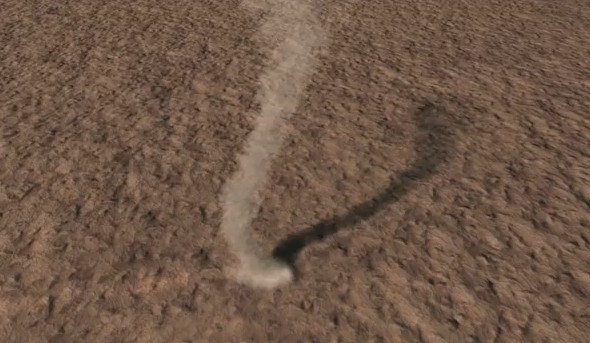
\includegraphics[scale=0.6]{fig/poussiere.jpg}}
  \caption{Dust Devil. Mars Reconnaissance Orbiter, made by HiRISE on Feb. 16, 2012}
  \label{fig:poussiere}
\end{figure}

Moreover, regarding the wind on Mars, in low altitudes, the Hadley circulation\footnote{movement on a planetary level of the layers of gases surrounding the planet} dominate and is almost the same process which, on Earth, generate the Trade winds. In high altitudes, a battery of areas of high and low pressure, named baroclinic pressure waves\footnote{In meteorology a baroclinic atmosphere is one for which the density depends on both the temperature and the pressure}, dominates the weather. The Mars wind lift a large amount of dust and can even trigger huge dust storms which can affect the while atmosphere (see Figure \ref{fig:storm}). Cyclonic storms can also appears on Mars. Indeed, cyclones similar to the ones of Earth tend to create during summer in the northern hemisphere but only in high latitudes.

\begin{figure}[h]
  \centerline{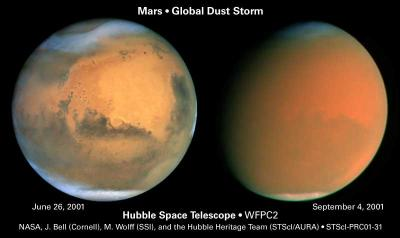
\includegraphics[scale=0.9]{fig/storm.jpg}}
  \caption{Two views of Mars with spatial telescope Hubble before and after the big dust storm in 2001}
  \label{fig:storm}
\end{figure}